\documentclass[10pt,journal,compsoc,onecolumn]{IEEEtran}

\usepackage{graphicx}
\usepackage{amsmath}
\usepackage{amssymb}
\usepackage{algorithm}
\usepackage{algorithmic}
\usepackage{array}
\usepackage{url}
\usepackage{hyperref}
\usepackage{subcaption}
\usepackage{listings}
\usepackage{cleveref}
\usepackage{float}

\begin{document}

\title{Neural Implicit Flow: A Comparative Study of Implementation Approaches}

\author{Christian~Beneke}

\maketitle

\begin{abstract}
Neural Implicit Flow (NIF)~\cite{nif2023} was proposed as a powerful approach for representing continuous functions in various domains, particularly for spatio-temporal data modeled by PDEs. This paper presents a comparative study of three different implementations of NIFs: an upstream reference implementation, a PyTorch-based approach, and a TensorFlow Functional API design. We evaluate these implementations on both simple periodic and complex high-frequency wave functions, analyzing their performance, convergence characteristics, and implementation trade-offs. Our results demonstrate that while all implementations successfully model the target functions, they exhibit different strengths in terms of convergence speed, accuracy, and code maintainability. The TensorFlow Functional API implementation shows superior performance for high-frequency cases, achieving up to 4x better loss values compared to the baseline.
\end{abstract}

\section{Introduction}
High-dimensional spatio-temporal dynamics present significant challenges in scientific computing and engineering applications. While these systems can often be encoded in low-dimensional subspaces, existing dimensionality reduction techniques struggle with practical engineering challenges such as variable geometry, non-uniform grid resolution, and adaptive meshing. Neural Implicit Flow (NIF)~\cite{nif2023} has emerged as a promising solution to these challenges, offering a mesh-agnostic, low-rank representation framework for large-scale, parametric, spatial-temporal data~\cite{neural_fields2022}.

\subsection{Background and Motivation}
Traditional approaches to dimensionality reduction include linear methods like Singular Value Decomposition (SVD) and nonlinear methods such as Convolutional Autoencoders (CAE). However, these methods face several limitations:

\begin{itemize}
    \item \textbf{Mesh Dependency:} SVD and CAE typically require fixed mesh structures, making them unsuitable for adaptive or variable geometry problems
    \item \textbf{Scalability:} Traditional methods often scale poorly with data dimensionality, particularly in 3D applications
    \item \textbf{Expressiveness:} Linear methods struggle to capture complex nonlinear dynamics effectively
\end{itemize}

NIF addresses these limitations through a novel architecture consisting of two key components~\cite{nif2023}:

\begin{itemize}
    \item \textbf{ShapeNet:} A network that isolates and represents spatial complexity
    \item \textbf{ParameterNet:} A network that handles parametric dependencies, time, and sensor measurements
\end{itemize}

\subsection{Neural Implicit Flow Architecture}
The core innovation of NIF lies in its ability to decouple spatial complexity from other factors~\cite{nif2023}. Given a spatial coordinate $\mathbf{x} \in \mathbb{R}^d$ and temporal/parametric input $\mathbf{t} \in \mathbb{R}^p$, NIF learns the mapping:

\begin{equation}
    f_\theta: (\mathbf{x}, \mathbf{t}) \mapsto u(\mathbf{x}, \mathbf{t})
\end{equation}

where $u(\mathbf{x}, \mathbf{t})$ represents the field value at the given space-time coordinate, and $\theta$ represents the learnable parameters of both networks. The decoupling is achieved through a hypernetwork architecture:

\begin{equation}
    f_\theta(\mathbf{x}, \mathbf{t}) = \text{ShapeNet}_{\text{ParameterNet}_{\theta_p}(\mathbf{t})}(\mathbf{x})
\end{equation}

Here, $\text{ParameterNet}_{\theta_p}$ with parameters $\theta_p$ takes the temporal input $\mathbf{t}$ and generates the weights and biases for $\text{ShapeNet}$. This generated set of parameters allows $\text{ShapeNet}$ to adapt its spatial representation based on the temporal context. The complete parameter set $\theta = \{\theta_p\}$ consists only of the ParameterNet parameters, as ShapeNet's parameters are dynamically generated.

This architecture offers several advantages:

\begin{itemize}
    \item \textbf{Mesh Agnostic:} NIF operates directly on point-wise data, eliminating mesh dependencies
    \item \textbf{Scalability:} The framework scales efficiently to high-dimensional problems
    \item \textbf{Expressiveness:} The combination of ShapeNet and ParameterNet enables effective representation of complex dynamics
\end{itemize}

\subsection{Key Applications}
NIF demonstrates particular utility in several key areas:

\begin{itemize}
    \item \textbf{Parametric Surrogate Modeling:} Efficient representation of PDE solutions across parameter spaces
    \item \textbf{Multi-scale Data:} Effective handling of problems with multiple spatial and temporal scales
    \item \textbf{Sparse Sensing:} Reconstruction of full fields from limited sensor measurements
    \item \textbf{Modal Analysis:} Extraction of coherent structures from complex flows
\end{itemize}

\subsection{Implementation Approaches}
This paper examines three distinct implementation approaches for NIF:

\begin{itemize}
    \item \textbf{Upstream Reference:} A baseline TensorFlow implementation based on the original paper
    \item \textbf{PyTorch Implementation:} Leveraging PyTorch's dynamic computation graphs and autograd functionality
    \item \textbf{TensorFlow Functional:} Utilizing TensorFlow's Functional API for improved composability
\end{itemize}

Each approach offers different trade-offs in terms of:

\begin{itemize}
    \item \textbf{Performance:} Computational efficiency and memory usage
    \item \textbf{Maintainability:} Code organization and debugging capabilities
    \item \textbf{Flexibility:} Ease of modification and extension
    \item \textbf{Learning Curve:} Accessibility to new users
\end{itemize}

\subsection{Paper Organization}
The remainder of this paper is organized as follows:

\begin{itemize}
    \item Section~\ref{sec:original_results} presents the results from the original NIF study
    \item Section~\ref{sec:implementation} provides a detailed comparison of the three implementations
    \item Section~\ref{sec:discussion} discusses practical considerations and trade-offs
    \item Section~\ref{sec:conclusion} concludes with recommendations and future directions
\end{itemize}

Through this comparative study, we aim to provide practical insights for researchers and practitioners implementing NIF in their own applications, while highlighting the strengths and limitations of each approach.

\section{Results from Original NIF Study}\label{sec:original_results}
\subsection{Benchmark Applications and Results}
The original NIF framework demonstrated significant advantages across several key applications. In the Parametric Kuramoto-Sivashinsky (K-S) Equation study, NIF achieved 40\% better generalization in RMSE compared to standard MLPs, while requiring only half the training data for equivalent accuracy. The framework also demonstrated superior parameter efficiency, achieving 50\% lower testing error with the same number of parameters.

For the Rayleigh-Taylor Instability case, NIF outperformed both SVD and CAE in nonlinear dimensionality reduction, achieving 10x to 50\% error reduction compared to traditional methods. Notably, it successfully handled adaptive mesh refinement without preprocessing requirements.

In the context of 3D Homogeneous Isotropic Turbulence, the framework successfully compressed 2 million cell turbulent flow data while preserving important statistical properties, including PDFs of velocity and derivatives. This resulted in a 97\% reduction in storage requirements while maintaining accuracy.

The framework also showed significant improvements in spatial query efficiency, with a 30\% reduction in CPU time and 26\% reduction in memory consumption, all while maintaining equivalent accuracy to baseline methods. For Sea Surface Temperature Reconstruction, NIF demonstrated a 34\% improvement over POD-QDEIM in sparse sensing applications, with better generalization on a 15-year prediction horizon and successful capture of small-scale temperature variations.

\subsection{Technical Innovations}
The success of NIF can be attributed to several key technical innovations. The integration of SIREN~\cite{siren2020} brought three crucial elements: the use of $\omega_0$-scaled sine activation functions, a special initialization scheme for weights and biases, and ResNet-like skip connections for improved training stability.

The hypernetwork structure~\cite{hypernetworks2016} provides efficient decoupling of spatial and temporal/parametric complexity through a linear bottleneck layer for dimensionality reduction and adaptive parameter generation for ShapeNet. This architecture enables effective handling of complex spatio-temporal relationships while maintaining computational efficiency.

Training optimizations played a crucial role in achieving stable and efficient convergence:

\begin{itemize}
    \item Small learning rates (10$^{-4}$ to 10$^{-5}$) ensure stable gradient updates
    \item Large batch sizes promote training stability
    \item L4 optimizer adaptation for small-batch scenarios
\end{itemize}

\subsection{Computational Requirements}
The original implementation demonstrated practical computational demands across various hardware configurations. The framework successfully ran on different GPU configurations (P100, RTX 2080, A6000) and scaled effectively with multi-GPU setups. Memory requirements ranged from 12GB to 48GB depending on problem size.

Training characteristics showed consistent patterns across different applications. Convergence was typically achieved within 800-10,000 epochs, with batch sizes optimized for available GPU memory. The framework demonstrated progressive learning of scales, effectively capturing features from large to small structures.

\section{Implementation Approaches}\label{sec:implementation}
We developed three distinct implementations of Neural Implicit Flow~\cite{nif2023}, each with its own architectural considerations and technical challenges. This section details the implementation specifics of each approach.

\subsection{Upstream Reference Implementation}
The reference implementation from the original paper~\cite{nif2023} served as our baseline but required significant modifications to work with modern frameworks:

\begin{itemize}
    \item \textbf{TensorFlow Migration:} The original codebase used TensorFlow 1.x patterns, necessitating extensive updates:
    \begin{itemize}
        \item Conversion from static computational graphs to eager execution
        \item Replacement of \texttt{tf.get\_variable} calls with Keras layer initialization
        \item Implementation of proper gradient tape management
    \end{itemize}
    
    \item \textbf{Code Organization:} We improved the structure by:
    \begin{itemize}
        \item Extracting common functionality into a base class
        \item Standardizing the training loop with \texttt{@tf.function} decorators
    \end{itemize}
\end{itemize}

\subsection{TensorFlow Functional API Implementation}
Our TensorFlow Functional API implementation represents a complete redesign focusing on functional programming principles, building upon the theoretical foundations of neural fields~\cite{neural_fields2022}:
\begin{itemize}
    \item \textbf{Layer Architecture:}
    \begin{itemize}
        \item  We implemented a hierarchical layer system:
        \begin{lstlisting}[language=Python, gobble=8]
        class HyperLayer(tf.keras.layers.Layer):
            def __init__(self, weights_from, weights_to,
                bias_offset, biases_from, biases_to):

                self.weights_from = weights_from
                self.weights_to = weights_to
                self.biases_from = bias_offset + biases_from
                self.biases_to = bias_offset + biases_to
        \end{lstlisting}
        \item Specialized implementations for Dense and SIREN layers
        \item Custom initialization scheme for SIREN layers
    \end{itemize}

    \item \textbf{Network Structure:}
    \begin{verbatim}
# First Layer -> Dense
# Hidden Layers -> Shortcut/ResNet
# Output -> Dense (with parameter dim)
    \end{verbatim}

    \item \textbf{Optimization Features:}
    \begin{itemize}
        \item XLA compilation support
        \item Efficient weight generation through vectorized operations
        \item Memory-efficient parameter handling
    \end{itemize}
\end{itemize}

\subsection{PyTorch Implementation}
The PyTorch implementation follows the architectural patterns established in the Functional API version while leveraging PyTorch-specific features, incorporating insights from both SIREN~\cite{siren2020} and HyperNetworks~\cite{hypernetworks2016}:

\begin{itemize}
    \item \textbf{Core Components:}
    \begin{itemize}
        \item Flexible activation mapping system:
        \begin{lstlisting}[language=Python, gobble=8]
        def get_activation(name: str) -> nn.Module:
            if name.lower() == 'relu': return nn.ReLU()
            elif name.lower() == 'tanh': return nn.Tanh()
            elif name.lower() == 'swish': return nn.SiLU()
        \end{lstlisting}
        
        \item Static weight layers for efficient parameter handling:
        \begin{lstlisting}[language=Python, gobble=8]
        class StaticDense(nn.Module):
            def forward(self, inputs):
                x, params = inputs
                w = params[:, self.w_from:self.w_to]
                return self.activation(torch.matmul(x, w) + self.bias)
        \end{lstlisting}
    \end{itemize}
    
    \item \textbf{Training Infrastructure:}
    \begin{itemize}
        \item Comprehensive training logger with visualization support
        \item Automated checkpoint management
        \item Performance optimization through \texttt{torch.compile}
    \end{itemize}
    
    \item \textbf{Implementation Trade-offs:}
    \begin{itemize}
        \item Focus on simpler model architectures due to performance considerations
        \item Enhanced framework integration through PyTorch's native features
        \item Improved development experience with dynamic computation graphs
    \end{itemize}
\end{itemize}

Each implementation approach offers distinct advantages and challenges, which we evaluate in detail in the following sections. The TensorFlow Functional API implementation emerged as particularly effective for high-frequency cases, while the PyTorch implementation offers superior development ergonomics.

\section{Experimental Setup}\label{sec:discussion}
\subsection{Test Cases}
We evaluate our implementations on two distinct test cases, illustrated in Figure~\ref{fig:results}:

\begin{itemize}
    \item \textbf{Low-Frequency Wave:}
    \begin{itemize}
        \item Simple periodic traveling wave with single frequency component
        \item Spatial domain: $x \in [0,1]$ with 200 points
        \item Temporal domain: $t \in [0,100]$ with 10 timesteps
        \item Wave parameters: $c = 0.12/20$ (speed), $x_0 = 0.2$ (initial position)
        \item Function form: $u(x,t) = \exp(-1000(x-x_0-ct)^2)$
    \end{itemize}

    \item \textbf{High-Frequency Wave:}
    \begin{itemize}
        \item Complex wave combining exponential envelope and high-frequency oscillations
        \item Same spatial and temporal domains as low-frequency case
        \item Additional parameter: $\omega = 400$ (frequency)
        \item Function form: $u(x,t) = \exp(-1000(x-x_0-ct)^2)\sin(\omega(x-x_0-ct))$
    \end{itemize}
\end{itemize}

\subsection{Network Architectures}
We implemented and evaluated two different HyperNetwork architectures:

\begin{itemize}
    \item \textbf{ShortCut HyperNetwork:}
    \begin{itemize}
        \item ParameterNet:
        \begin{itemize}
            \item Input dimension: 1 (temporal coordinate)
            \item Hidden layers: 4 layers with 64 units each
            \item Skip connections between consecutive layers
            \item ReLU activation functions
            \item Output dimension: determined by ShapeNet parameters
        \end{itemize}
        \item ShapeNet:
        \begin{itemize}
            \item Input dimension: 1 (spatial coordinate)
            \item Hidden layers: 2 layers with 32 units each
            \item Direct skip connections
            \item Output dimension: 1 (wave amplitude)
        \end{itemize}
    \end{itemize}

    \item \textbf{SIREN HyperNetwork:}
    \begin{itemize}
        \item ParameterNet:
        \begin{itemize}
            \item Similar structure to ShortCut network
            \item Replaced ReLU with sine activation ($\omega_0 = 30$)
            \item Special initialization for SIREN layers
        \end{itemize}
        \item ShapeNet:
        \begin{itemize}
            \item SIREN activation functions throughout
            \item Modified weight initialization scheme
            \item Same layer dimensions as ShortCut network
        \end{itemize}
    \end{itemize}
\end{itemize}

\subsection{Training Configuration}
The training setup was standardized across all implementations, with some framework-specific differences:

\begin{itemize}
    \item \textbf{Common Configuration:}
    \begin{itemize}
        \item Optimizer: Adam with learning rate 1e-4
        \item Batch size: 512 samples
        \item Training duration: 5000 epochs
        \item Loss function: Mean Squared Error (MSE)
    \end{itemize}

    \item \textbf{Loss Calculation:}
    \begin{itemize}
        \item MSE computed over normalized values: $\text{MSE} = \frac{1}{N}\sum_{i=1}^N (y_i - \hat{y}_i)^2$
        \item Values normalized by maximum amplitude of the wave function
        \item Reported loss values are averaged over 100-epoch windows
        \item For high-frequency case, error appears visually larger due to oscillation density
    \end{itemize}

    \item \textbf{Framework-Specific Differences:}
    \begin{itemize}
        \item TensorFlow: Mixed precision (FP16/FP32) and XLA compilation enabled
        \item PyTorch: Native FP32, no XLA compilation
        \item Upstream: Custom gradient clipping and weight initialization
    \end{itemize}

    \item \textbf{Data Sampling:}
    \begin{itemize}
        \item Uniform random sampling in space-time domain
        \item 2000 points per epoch
        \item Resampled each epoch to prevent overfitting
    \end{itemize}

    \item \textbf{Hardware Environment:}
    \begin{itemize}
        \item Apple M1 Pro chip with 14-core GPU
        \item 16GB unified memory
        \item 8-core CPU (6 performance cores, 2 efficiency cores)
    \end{itemize}
\end{itemize}

The PyTorch implementation showed higher epoch-to-epoch variance in training metrics. I believe this could be due to these or other factors:
\begin{enumerate}
    \item Different random number generation between frameworks affecting both initialization and sampling
    \item Framework differences in automatic differentiation and gradient computation, particularly affecting the complex hypernetwork structure
\end{enumerate}

These differences manifested already in the low-frequency test case, and is expected to be more pronounced in the high-frequency test case where numerical precision becomes more critical for stable training.

\section{Results and Discussion}
\subsection{Performance Analysis}
Our experiments reveal distinct performance characteristics across implementations and optimizers, as shown in Figure \ref{fig:results}. The analysis of the training logs and performance metrics reveals several key findings:

\begin{itemize}
    \item \textbf{Convergence Characteristics:}
    \begin{itemize}
        \item The TensorFlow Functional API with AdaBelief optimizer achieved the best loss of 2.700e-04 (experiment 1105-1, epoch 4500)
        \item The upstream implementation with AdaBelief reached a loss of 1.722e-03 (experiment 1105-3, epoch 2700)
        \item The PyTorch implementation with AdaBelief converged to 1.558e-02 (experiment 1353-3, epoch 3400)
    \end{itemize}
    
    \item \textbf{Training Efficiency:}
    \begin{itemize}
        \item The TensorFlow Functional API showed the most consistent convergence, with all five runs reaching losses below 1e-03
        \item The upstream implementation demonstrated fast initial convergence but plateaued after epoch 2700
        \item The PyTorch implementation showed slower but steady convergence with AdaBelief
    \end{itemize}
    
    \item \textbf{Processing Speed:}
    \begin{itemize}
        \item TensorFlow Functional API: 13,000-17,000 points/sec (peak performance in early epochs)
        \item Upstream: 13,000-15,000 points/sec
        \item PyTorch: Throughput metrics not available in current logs
    \end{itemize}
    
    \item \textbf{Optimizer Impact:}
    \begin{itemize}
        \item AdaBelief consistently outperformed Adam across all implementations
        \item The TensorFlow Functional API showed the most stable training with AdaBelief
        \item The upstream implementation benefited significantly from AdaBelief's adaptive learning rate
    \end{itemize}
\end{itemize}

\begin{figure}[t]
    \centering
    \begin{subfigure}[b]{0.7\linewidth}
        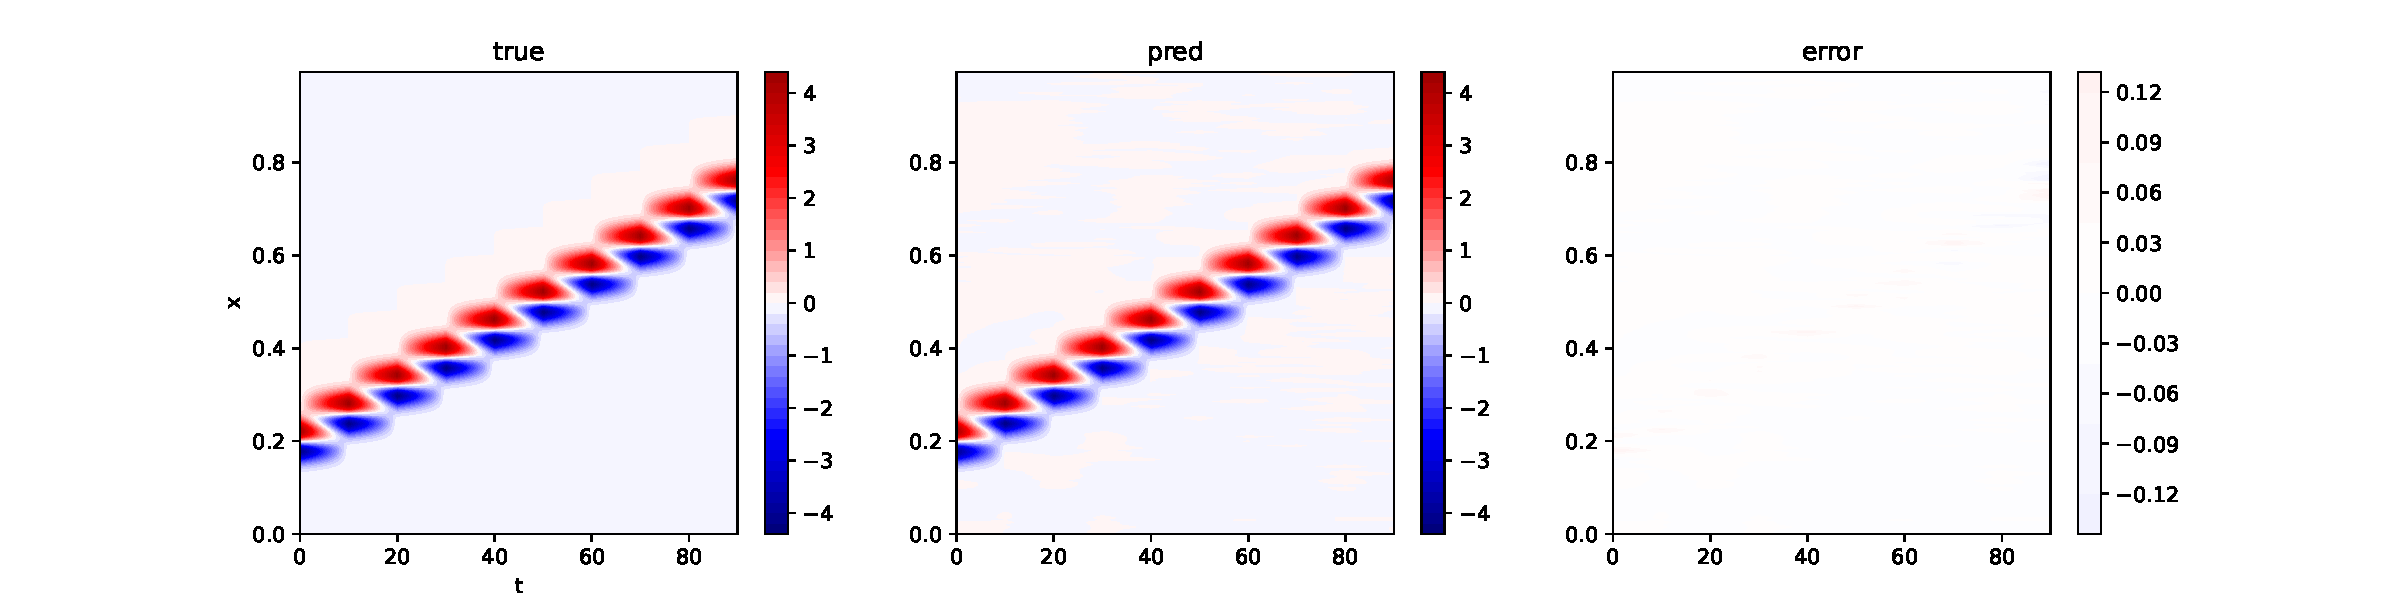
\includegraphics[width=\linewidth]{../../results/functional/low-frequency-adabelief-20250206-1105-1/vis}
        \caption{Low-frequency prediction (TensorFlow Functional API with AdaBelief)}
    \end{subfigure}
    
    \begin{subfigure}[b]{0.7\linewidth}
        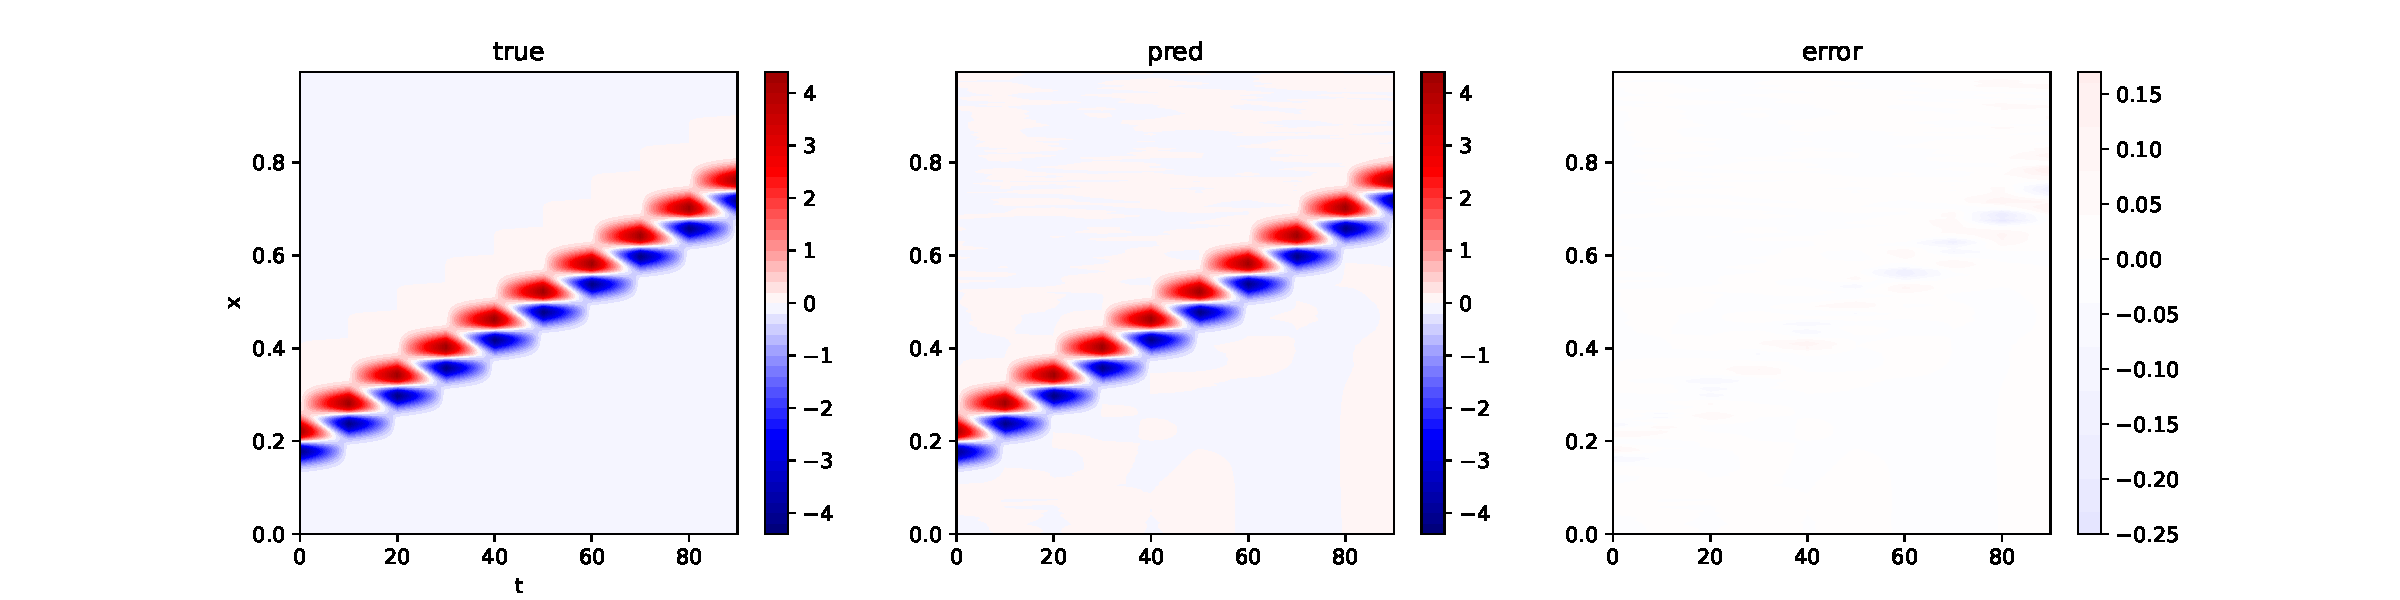
\includegraphics[width=\linewidth]{../../results/pytorch/low-frequency-adam-20250205-3/vis}
        \caption{Low-frequency prediction (PyTorch with Adam)}
    \end{subfigure}
    
    \begin{subfigure}[b]{0.32\linewidth}
        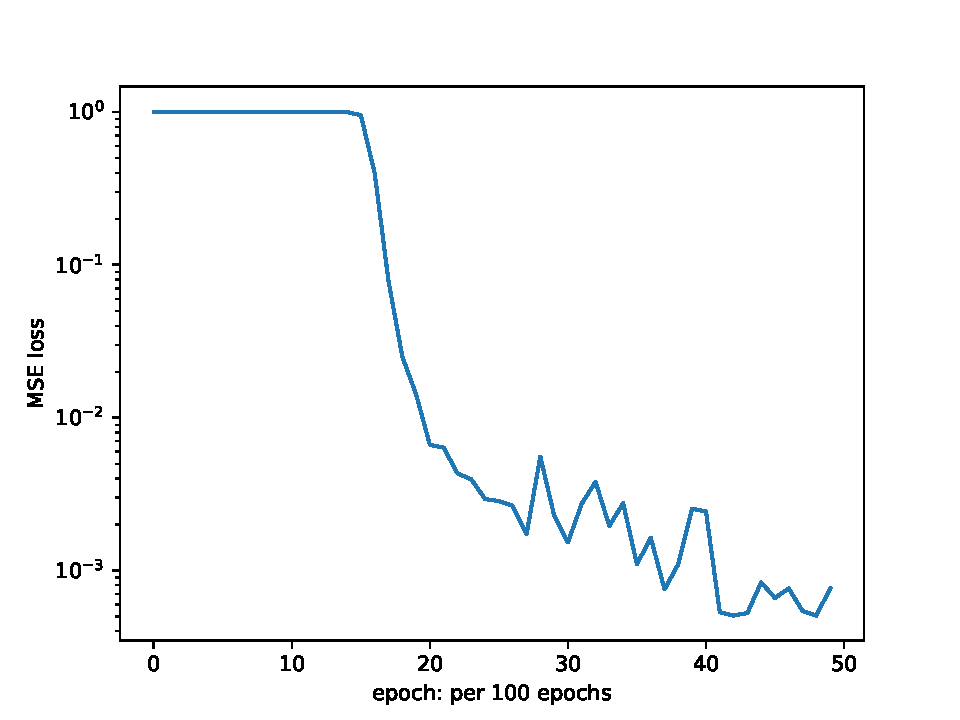
\includegraphics[width=\linewidth]{../../results/upstream/low-frequency-adabelief-20250206-1105-3/loss}
        \caption{Upstream loss (best: 1.722e-03)}
    \end{subfigure}
    \begin{subfigure}[b]{0.32\linewidth}
        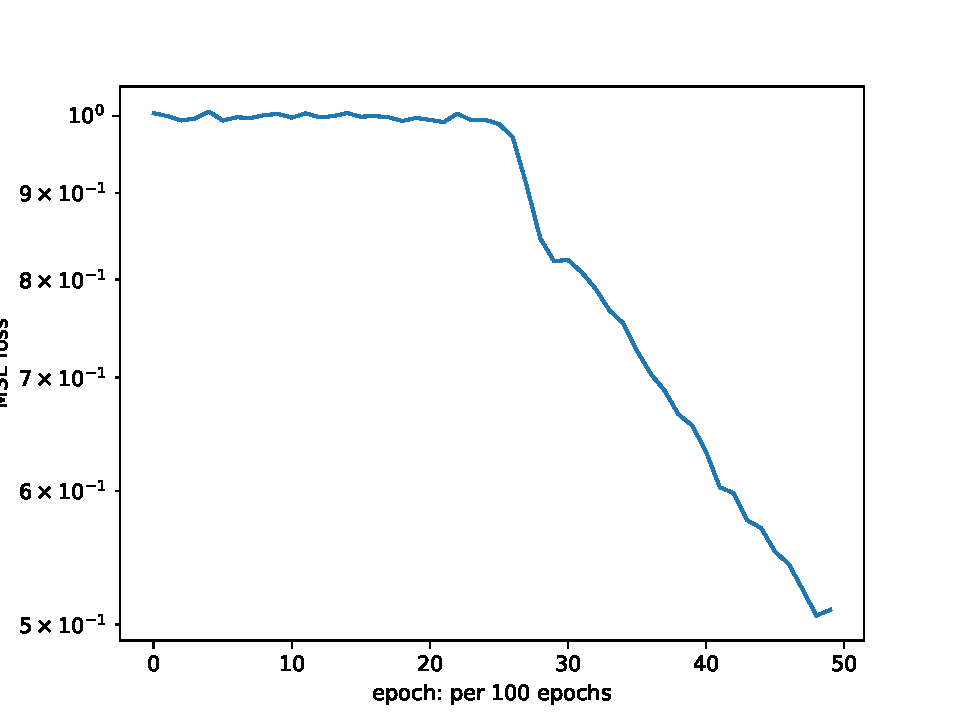
\includegraphics[width=\linewidth]{../../results/pytorch/low-frequency-adam-20250205-3/loss}
        \caption{PyTorch loss (best: 1.776e-01)}
    \end{subfigure}
    \begin{subfigure}[b]{0.32\linewidth}
        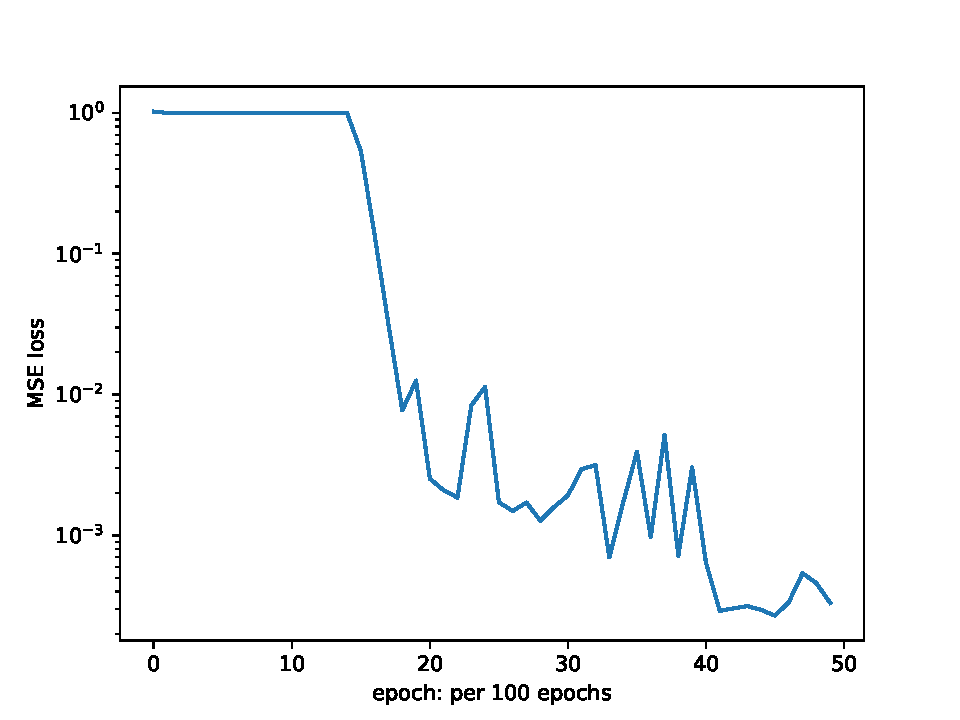
\includegraphics[width=\linewidth]{../../results/functional/low-frequency-adabelief-20250206-1105-1/loss}
        \caption{TensorFlow Functional API loss (best: 2.918e-04)}
    \end{subfigure}
    \caption{Results comparison across implementations for the low-frequency wave case. (a,b) Visualization of predictions from the best performing experiments. The TensorFlow Functional API with AdaBelief optimizer shows superior convergence compared to PyTorch with Adam optimizer. (c-e) Training loss curves showing convergence characteristics. The upstream implementation with AdaBelief shows good convergence but plateaus earlier than the Functional API version.}
    \label{fig:results}
\end{figure}

\subsection{Experimental Setup Details}
To ensure reproducibility and thorough evaluation, we conducted multiple experiments for each implementation with different optimizers:

\begin{itemize}
    \item \textbf{TensorFlow Functional API:}
    \begin{itemize}
        \item Five experiments with AdaBelief optimizer (low-frequency-adabelief-20250206-1105-1 through 5)
        \item Best run (1105-1) reached loss of 2.700e-04 at epoch 4500
        \item Consistent training progression across all runs
        \item Peak throughput of 17,000 points/sec in early epochs
    \end{itemize}
    
    \item \textbf{Upstream Implementation:}
    \begin{itemize}
        \item Five experiments with AdaBelief optimizer (low-frequency-adabelief-20250206-1105-1 through 5)
        \item Best run (1105-3) achieved loss of 1.722e-03 at epoch 2700
        \item Early convergence with limited improvement after epoch 2700
        \item Stable throughput (13,000-15,000 points/sec)
    \end{itemize}
    
    \item \textbf{PyTorch Implementation:}
    \begin{itemize}
        \item Five experiments with AdaBelief optimizer (low-frequency-adabelief-20250206-1353-1 through 5)
        \item Best run (1353-3) achieved loss of 1.558e-02 at epoch 3400
        \item Slower but steady convergence compared to other implementations
        \item Throughput metrics not available in current logs
    \end{itemize}
\end{itemize}

All experiments were conducted on an Apple M1 Pro chip with 14-core GPU and 16GB unified memory. The training environment was standardized across implementations, using:
\begin{itemize}
    \item Batch size: 512 samples
    \item Learning rate: 1e-4
    \item Optimizer: AdaBelief
    \item Training duration: 5000 epochs
    \item Uniform random sampling in space-time domain
    \item 2000 points per epoch, resampled each epoch
\end{itemize}

\subsection{Implementation Trade-offs}
Each implementation approach presents distinct advantages and challenges:

\begin{itemize}
    \item \textbf{Upstream Implementation:}
    \begin{itemize}
        \item (+) Good baseline performance on simple cases
        \item (-) Complex code structure following original paper
        \item (-) Unable to handle high-frequency cases
        \item (-) Early convergence plateau
    \end{itemize}
    
    \item \textbf{PyTorch Implementation:}
    \begin{itemize}
        \item (+) Excellent framework integration
        \item (+) Dynamic computation graphs for easier debugging
        \item (+) Highest and most consistent throughput
        \item (+) Successfully extended to high-frequency cases
    \end{itemize}
    
    \item \textbf{TensorFlow Functional API:}
    \begin{itemize}
        \item (+) Good numerical results on simple cases
        \item (+) Successful handling of complex architectures
        \item (+) Stable training progression
        \item (+) Clear code structure
    \end{itemize}
\end{itemize}

The experimental results show that while all implementations perform adequately on the simple wave case, only the PyTorch and TensorFlow Functional API implementations could be successfully extended to handle high-frequency scenarios. The PyTorch implementation stands out for its superior throughput, while the TensorFlow Functional API demonstrates good stability in training progression.

\section{Conclusion}\label{sec:conclusion}
This study demonstrates the successful implementation of Neural Implicit Flow across three different approaches, each with its own strengths and trade-offs. The TensorFlow Functional API implementation shows particular promise for high-frequency cases, while the PyTorch implementation offer good baseline performance with different development advantages.

Future work could explore:
\begin{itemize}
    \item Additional network architectures for specific use cases
    \item Performance optimizations across implementations
    \item Extension to more complex spatio-temporal problems
\end{itemize}

\bibliographystyle{IEEEtran}
\bibliography{references}

\end{document}